\selectlanguage{australian}%
%\begin{landscape}


\chapter{\label{chap:Apx-Data}Data}


\section{Data Congregated from Literature\label{sec:litresults}}

%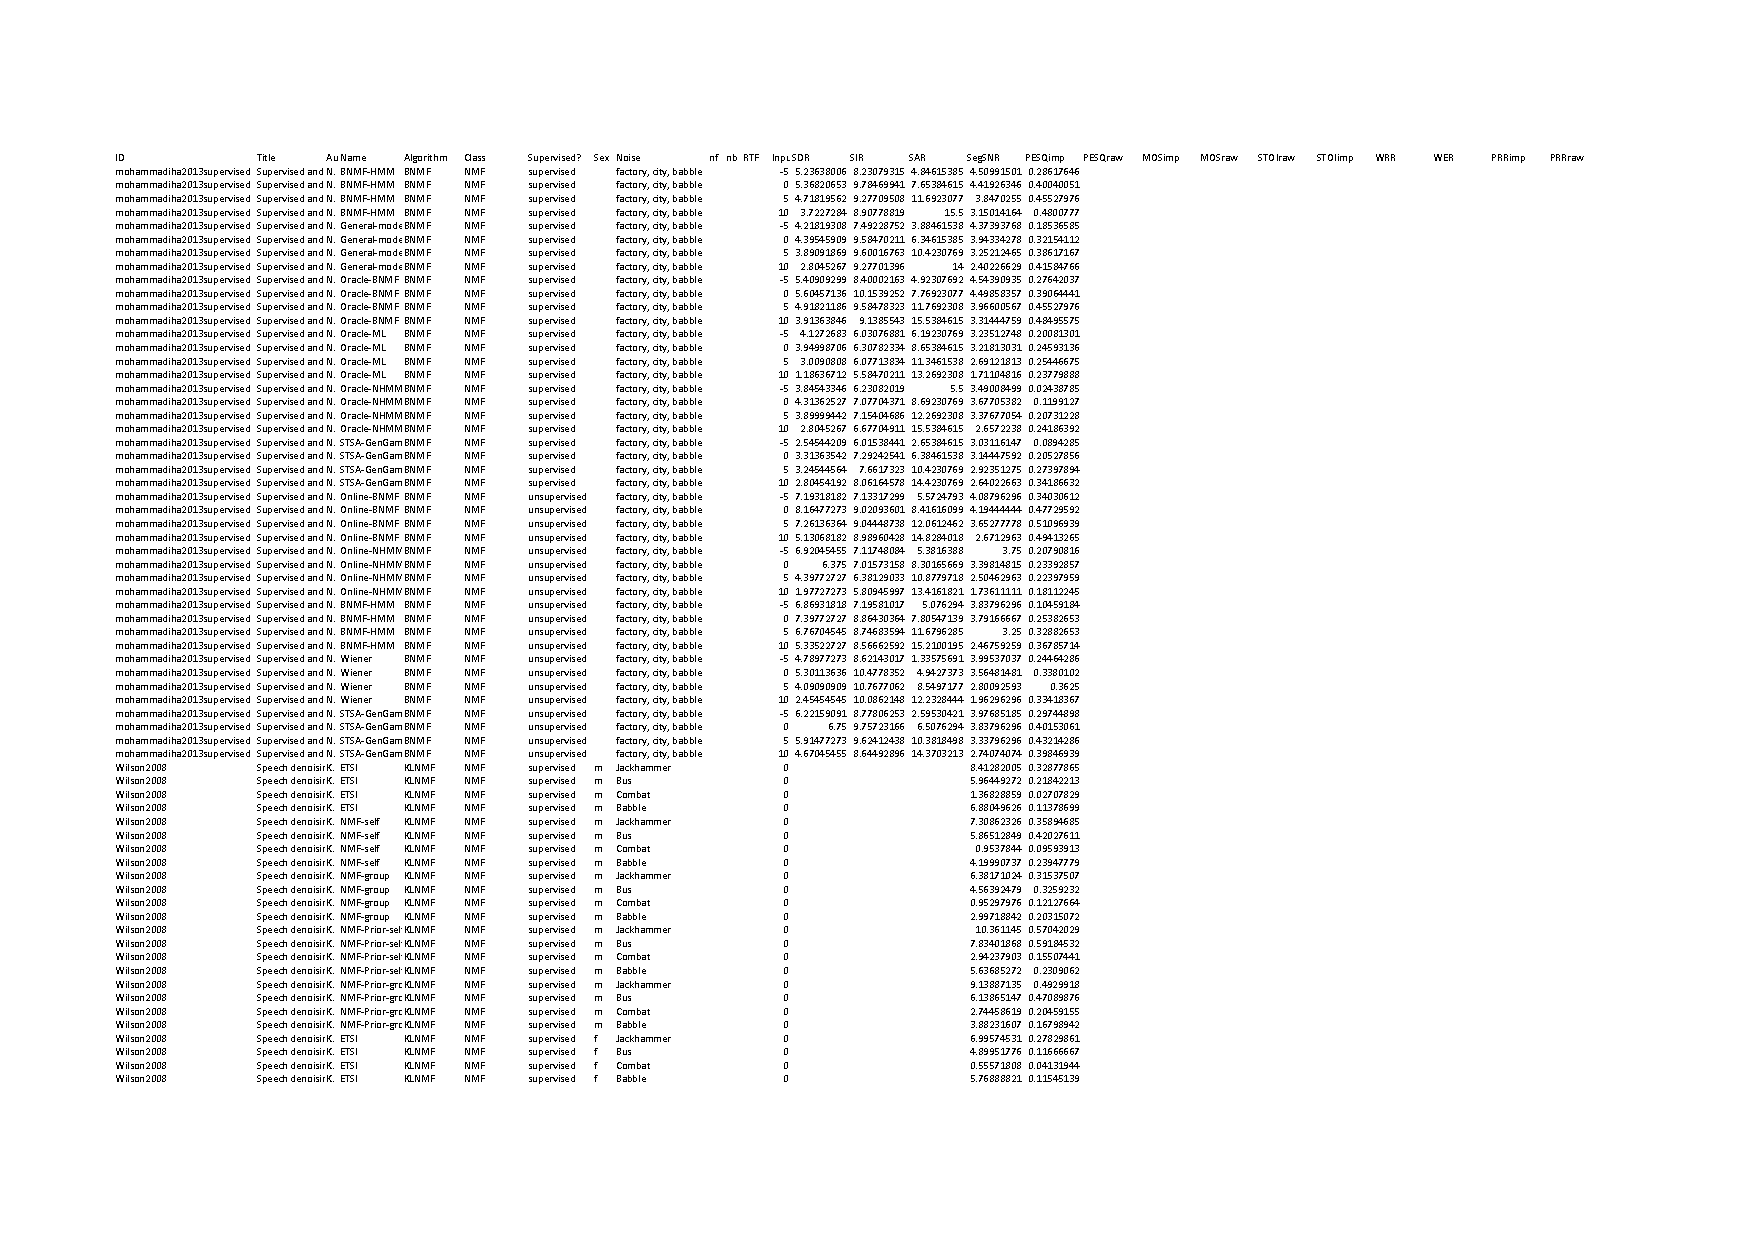
\includepdf[pages=-,angle=90]{dat/litresults}

%\end{landscape}

Just file ref?


\chapter{Code}


\section{MATLAB Test Code}

\lstset{style=Matlab-editor,basicstyle=\mlttfamily\small,title=\lstname}

\begin{listing}[H]
\protect\caption{Create Test Data MATLAB Code\label{lst:createTestData}}


\lstinputlisting[lastline=46]{../Code/MATLAB/Test/createTestData.m}
\end{listing}


\lstinputlisting[firstline=47,firstnumber=last]{../Code/MATLAB/Test/createTestData.m}

\begin{listing}[H]
\protect\caption{``Varying Training'' Test MATLAB Code\label{lst:varyingTrainingTest}}


\lstinputlisting[lastline=53]{../Code/MATLAB/Test/varyingTrainingTest.m}
\end{listing}


\lstinputlisting[firstline=54,firstnumber=last]{../Code/MATLAB/Test/varyingTrainingTest.m}

\begin{listing}[H]
\protect\caption{``Varying Training'' Analysis MATLAB Code\label{lst:varyingTrainingAnalysis}}


\lstinputlisting[lastline=53]{../Code/MATLAB/Test/varyingTrainingAnalysis.m}
\end{listing}


\lstinputlisting[firstline=54,firstnumber=last]{../Code/MATLAB/Test/varyingTrainingAnalysis.m}


\section{R Analysis Code}

\lstset{ language=R,% set programming language
         title=\lstname,
         basicstyle=\small\ttfamily,% basic font style
         keywordstyle=\color{blue},% keyword style
         commentstyle=\ttfamily\itshape\color{gray},% comment style
         numbers=left,% display line numbers on the left side
         numberstyle=\scriptsize\color{gray},% use small line numbers
         numbersep=10pt,% space between line numbers and code
         tabsize=2,% sizes of tabs
         showstringspaces=false,% do not replace spaces in strings by a certain character
%         captionpos=b,% positioning of the caption below
         breaklines=true,% automatic line breaking
         escapeinside={(*}{*)},% escaping to LaTeX
%         fancyvrb=true,% verbatim code is typset by listings
         extendedchars=false,% prohibit extended chars (chars of codes 128--255)
         literate={<-}{{$\leftarrow$}}1{<<-}{{$\twoheadleftarrow$}}1
         {~}{{$\sim$}}1{<=}{{$\le$}}1{>=}{{$\ge$}}1{!=}{{$\neq$}}1{^}{{$^\wedge$}}1,% item to replace, text, length of chars
         alsoletter={.<-},% becomes a letter
         alsoother={$},% becomes other
         otherkeywords={!=, ~, $, *, \&, \%/\%, \%*\%, \%\%, <-, <<-},% other keywords
         stringstyle=\color{dkgreen},
         deletekeywords={c, /}% remove keywords
}

\begin{listing}[H]
\protect\caption{Direct Comparison R Code\label{lst:directComp}}


\lstinputlisting[lastline=50]{../Code/R/directComp.R}
\end{listing}


\lstinputlisting[firstline=51,firstnumber=last]{../Code/R/directComp.R}

\begin{listing}[h]
\protect\caption{Indirect Comparison R Code\label{lst:indirectComp}}


\lstinputlisting[language=R]{../Code/R/indirectComp.R}

\selectlanguage{english}%
\selectlanguage{english}%
\end{listing}
\selectlanguage{english}%

